\section{Telemedicina}

La Telemedicina \cite{aim}, \cite{bashshur77}, \cite{itu} se ha convertido rápidamente en un concepto que extiende sus raices etimológicas. El Ministerio de Protección Social colombiano con la \textit{Resolución 1448 del 8 de mayo de 2006} define a la Telemedicina como:
\begin{quote}
“la provisión de servicios de salud a distancia, en los componentes de promoción, prevención, diagnóstico, tratamiento o rehabilitación, por profesionales de la salud que utilizan tecnologías de la información y la comunicación, que les permiten intercambiar datos con el propósito de facilitar el acceso de la población a servicios que presentan limitaciones de oferta, de acceso a los servicios o de ambos en su área geográfica.”
\end{quote} 

Es por tanto un campo multidisciplinar que integra componentes de diferentes áreas del saber que incluye entre otros a la medicina, la ingeniería electrónica, la telemática, la informática, la ingeniería de sistemas, la inteligencia artificial, la biónica, la sicología, la sociología y la antropología. Las redes actuales de Telemedicina consideran elementos que van mucho más alla del simple despliegue de redes tecnológicas de intercomunicación y evidentemente se plantean como redes de interacción social cuyo objetivo primario - más no el único, es la prestación de servicios médicos apoyadas en las TIC.

Dependiendo el grado en que se presente cada uno de los elementos mostrados en la figura ~\ref{elementosred} y de la mayor o menor correlación entre ellos, se pueden crear sistemas de Telemedicina que se acerquen al ideal de proveer servicios de salud de alta calidad. Dichos sistemas, aunque dinámicos y evolutivos, deberán mantener una estructura nuclear cuyas propiedades generales son según \cite{bashshur95}: 
\begin{enumerate}
\item Separación geográfica entre el proveedor y el cliente durante un encuentro clínico o entre dos o más proveedores.
\item Utilización de tecnologías informáticas y de comunicaciones para realizar la interacción. 
\item Equipo humano/técnico de gestión del sistema. 
\item Desarrollo de una infraestructura organizacional. 
\item Desarrollo de protocolos clínicos para orientar a los pacientes hacia diagnósticos y fuentes de tratamiento apropiados. 
\item Normas de comportamiento que reemplazan las normas del comportamiento presenciales.
\end{enumerate}

\begin{figure}
 \centering
 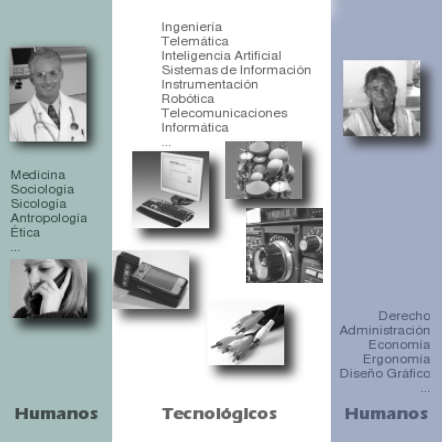
\includegraphics[width=156mm, height=156mm]{sistema_telemedicina.png}
 \caption{Elementos genéricos y áreas del saber de una red de Telemedicina}
 \label{elementosred}
\end{figure}

La Telemedicina es catalogada siguiendo básicamente criterios de \cite{oas2002}: sincronización temporal entre el proveedor y el cliente -diferida o en tiempo real; servicios de salud que se presten \cite{aparicio2000} - consulta, diagnóstico, atención, seguimiento, educación, administración, etc;  o especialidad médica que se trate - radiología, patología, cardiología, dermatología, etc. La catalogación siempre es independiente de la red tecnológica y de comunicaciones sobre la cual se despliegue.

\subsection{Componentes Tecnológicos de los Sistemas de Telemedicina}
La fase actual del SITEM se centra en dos conjuntos básicos de componentes de los sistemas de Telemedicina, los médicos y los tecnológicos. Debido al perfil de profesionales que han participado en el desarrollo, los elementos tecnológicos han sido mejor caracterizados hasta el momento.

\begin{figure}
 \centering
 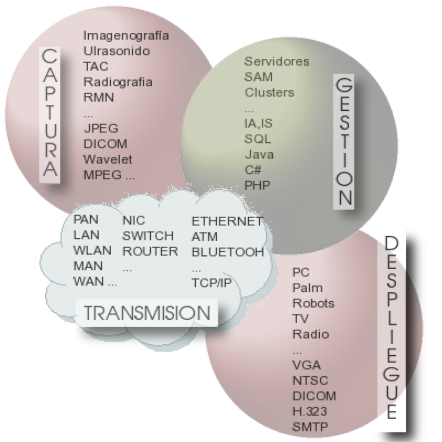
\includegraphics[width=156mm, height=156mm]{red_1.png}
 \caption{Subsistemas Tecnológicos Básicos en un Sistema de Telemedicina}
 \label{subsistemas}
\end{figure}


Para efectos de facilitar su análisis y modelado, en la dimensión puramente tecnológica, un sistema de Telemedicina puede reducirse a cuatro subsistemas \cite{aparicio2003}:

\begin{itemize}
 \item \textbf{Captura de datos:} Conformado por los dispositivos de hardware, los protocolos y aplicaciones software que trabajan conjuntamente para transformar información médica en datos susceptibles de ser administrados usando técnicas digitales.
 \item \textbf{Transmisión de Datos:} Hacen parte de este subsistema los dispositivos de hardware, las tecnologías de interconexión, los protocolos y aplicaciones que permiten estructurar redes de transmisión de datos digitales de una manera fiable en tiempos aceptables para un servicio específico.
 \item \textbf{Gestión de Información:} Dispositivos de hardware - computadores, sistemas de almacenamiento masivo, etc; y  sistemas de información que almacenan, procesan, distribuyen y analizan la información proveniente de los subsistemas de captura de datos.
 \item \textbf{Despliegue de información:} Elementos de hardware (pantallas, transductores, sistemas de audio, etc), aplicaciones software y protocolos asociados que permiten recibir y reproducir la información médica. 
\end{itemize}

Todos ellos necesariamente interrelacionados por medio de interfaces y protocolos definidos; El uso de estándares abiertos es de vital importancia para permitir que los sistemas de Telemedicina puedan ser interoperables, esto se ha logrado en gran medida en el subsistema de transmisión de datos pero aún se encuentran serios problemas en los demás subsistemas debido al sinnúmero de patentes y protocolos propietarios que las empresas fabricantes de dispositivos médicos aún ostentan.